%versi 3 (22-07-2020)
\chapter{Analisis}
\label{chap:analisis}
Pada bab ini akan membahas mengenai proses pengumpulan data citra satelit yang berada di Laboratium Fakultas Tenik Informatika dan Sains(FTIS) UNPAR(Universitas Katolik Parahyangan) beserta gambar citra satelit segmentasi, pengambilan data dari hasil penelitian yang telah dilakukan oleh Juan A. Kusnandji, dan analisis kebutuhan perangkat lunak dalam pengembangan halaman web.

\section{Proses Pembentukan Gambar}
Pada Gambar \ref{fig:ciumbuleuit3} merupakan hasil dari penggabungan gambar per \textit{tile}. Langkah-langkah dalam proses pengambilan data berupa gambar citra satelit dari kelurahan di Kota Bandung. 
\begin{figure}[H]
	\centering
	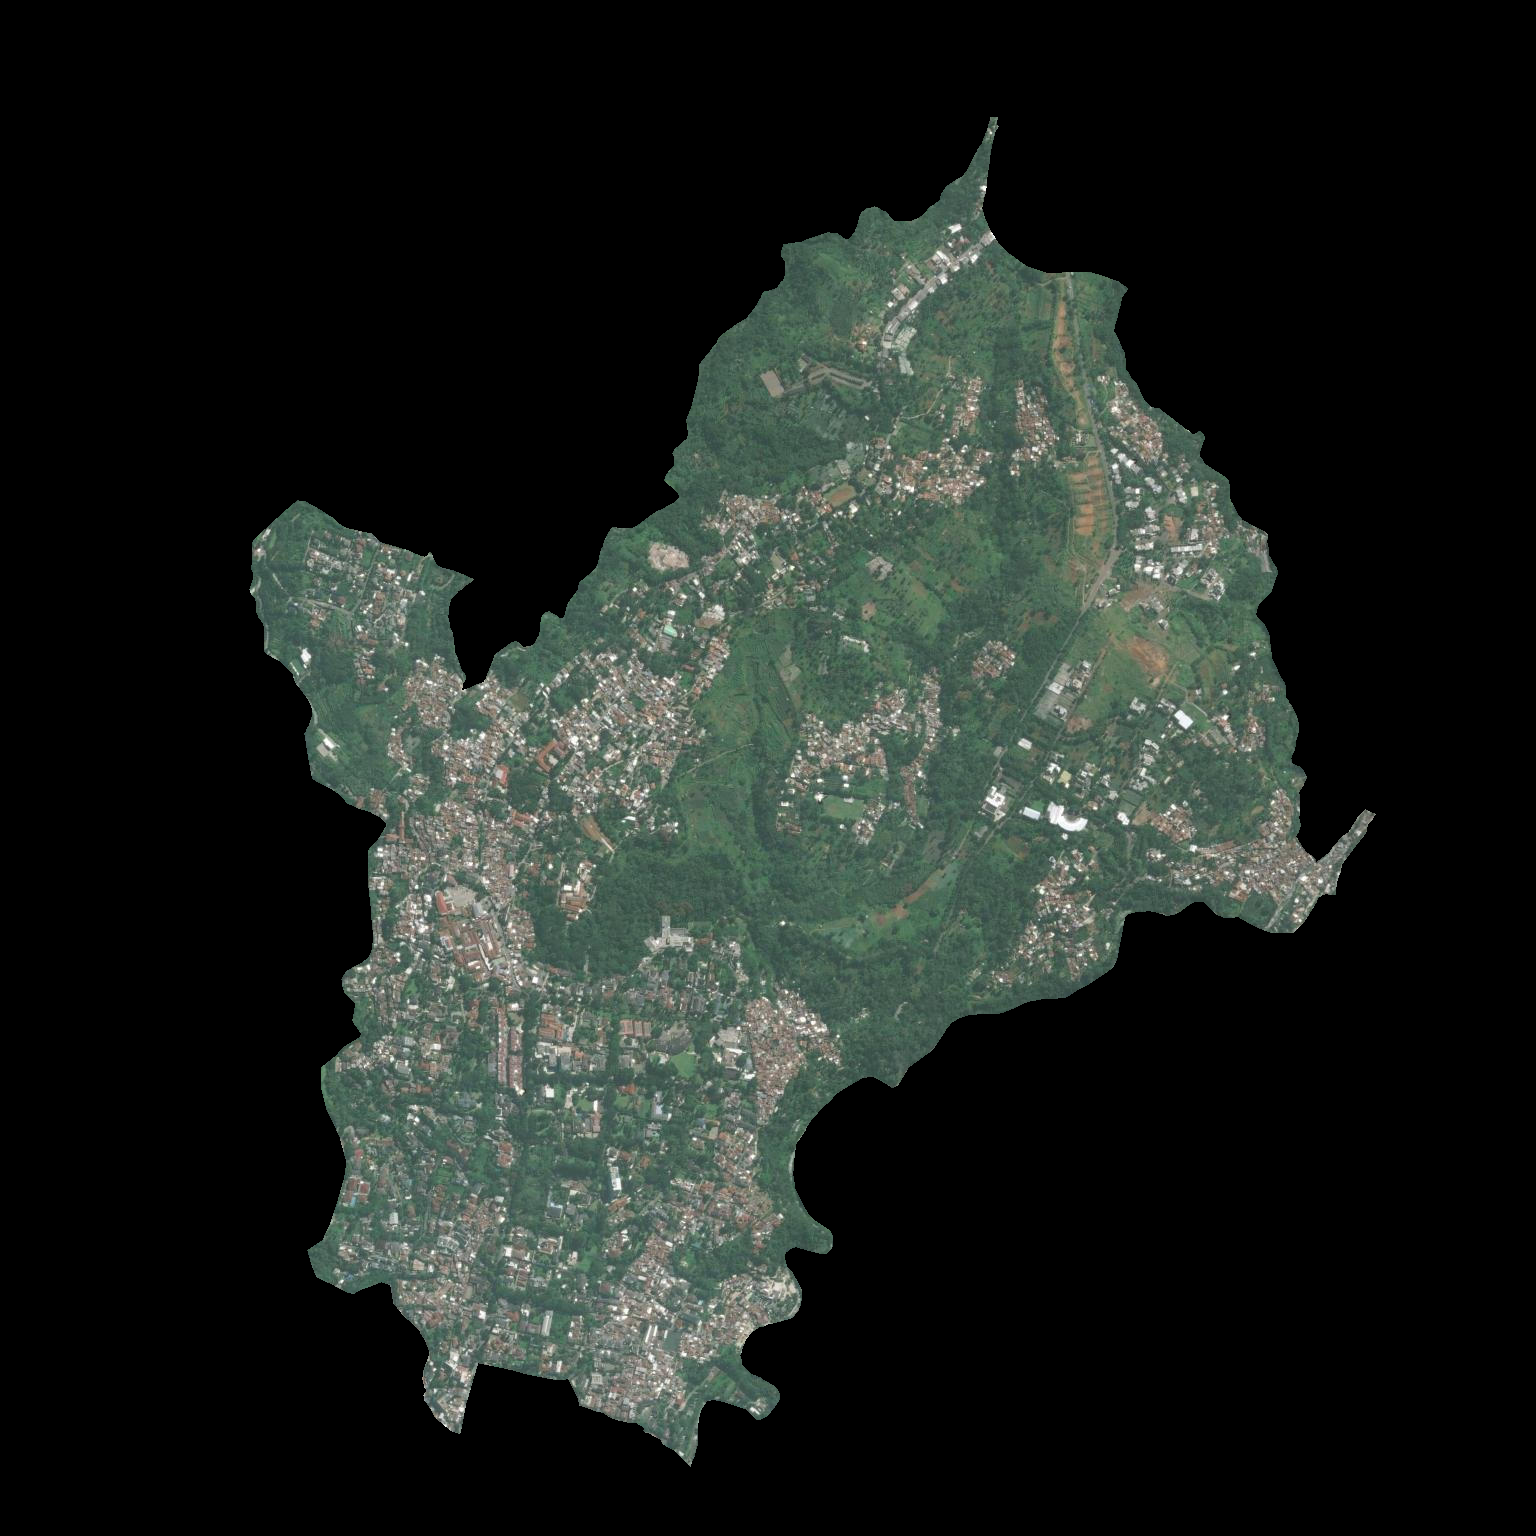
\includegraphics[width=0.5\textwidth]{Gambar/Ciumbuleuit.png}
	\caption{Gambar seluruh tile dari kelurahan Ciumbuleuit}
	\label{fig:ciumbuleuit3}
\end{figure} 

Proses awal dilakukan meliputi data yang diambil dari sistem Hadoop yang disimpan pada Hadoop Laboratoium FTIS UNPAR. Kemudian data yang telah diambil berupa file ".txt" yang setiap baris dari file tersebut merupakan sebuah file gambar berupa \textit{tile} seperti pada gambar(\ref{fig:tileCiumbuleuit}). Kumpulan gambar per \textit{tile} akan digabungkan dengan menggunakan \textit{script}. Penggabungan gambar setiap \textit{tile} akan menghasilkan sebuah gambar dari kelurahan seperti pada gambar \ref{fig:ciumbuleuit}.
\begin{figure}[H]
	\centering
	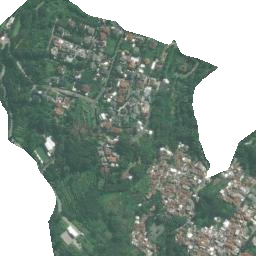
\includegraphics[scale=0.4]{Ciumbuleuit21.png}
	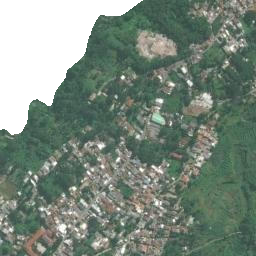
\includegraphics[scale=0.4]{Ciumbuleuit22.png}
	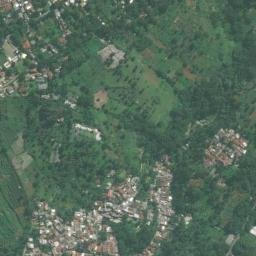
\includegraphics[scale=0.4]{Ciumbuleuit23.png}
	\caption{Contoh gambar kelurahan Ciumbuleuit setiap \textit{tile}}
	\label{fig:tileCiumbuleuit}
\end{figure}

\subsection{Mengunduh File Text}

Pada penelitian yang telah dilakukan oleh Juan Anthonius Kusjadi menghasilkan data yang telah disimpan pada sistem \textit{data lake }yang telah dibuat pada HDFS.\cite{juan:22:pengumpulan} Pada proses pengunduhan data harus terlebih dahulu mendaftarkan akun HDFS pada admin laboratoium FTIS UNPAR agar mendapat akses kedalam sistem penyimpanan HDFS(\textit{Hadoop Distributed File System}). Setelah mendapatkan aksesnya, lalu dapat mengunduh data citra satelit kelurahan per kota dengan perintah seperti pada kode \ref{code:cmdhdfs}. 

\begin{lstlisting}[language=Bash, caption=\textit{Command-line} HDFS,label={code:cmdhdfs}]
	hdfs dfs -get /user/if18059/geodata/cropped/arcgis/16/Jawa_Barat/Kota_Bandung.txt .	
\end{lstlisting}

Metode yang umum digunakan untuk mengunduh file dari server jarak jauh secara aman adalah dengan menggunakan SCP (\textit{Secure Copy Protocol}). SCP adalah perintah baris perintah yang memungkinkan pengguna untuk mentransfer file antara komputer lokal dan server jarak jauh melalui koneksi yang aman. Dalam pengunduhan file dari server dapat menggunakan perintah 'scp' diikuti oleh alamat sumber file di server dan alamat tujuan pada penyimpanan lokal. Dapat dilihat pada \textit{command-line} \ref{code:cmdscp}, akan mengunduh file 'Kota\_Bandung.txt' dari server HDFS laboratorium FTIS UNPAR ke lokasi yang ditentukan pada penyimpanan lokal. Dengan demikian, File yang telah diunduh dapat dengan mudah digunakan.

\begin{lstlisting}[language=Bash, caption=\textit{Command-line} SCP,label={code:cmdscp}]
	C:\Users\Asus>scp ssh i17086@10.100.69.101:Kota_Bandung.txt	
\end{lstlisting}

Data Kota\_Bandung.txt dapat dilihat pada gambar \ref{fig:kotabandungteks}. Isi dari berkas Kota\_Bandung.txt memiliki 9 kolom yang dipisahkan oleh tanda titik koma (”;”). Pada kolom pertama diisi dengan nama kelurahan. Pada kolom kedua diisi dengan nama kota. Pada kolom ketiga diisi dengan nama provinsi. Kolom keempat diisi dengan nilai panjang tile untuk kelurahan tersebut. Kolom kelima diisi dengan nilai lebar dari tile untuk kelurahan tersebut. Kolom keenam diisi dengan posisi x koordinat tile untuk kelurahan tersebut. Kolom ketujuh diisi dengan posisi y koordinat tile untuk kelurahan tersebut. Kolom kedelapan diisi dengan ukuran luas per piksel dalam km2 untuk tile pada kelurahan tersebut. Terakhir kolom kesembilan diisi dengan data
tile citra satelit dengan format png yang sudah dienkripsi dalam bentuk Base64\cite{juan:22:pengumpulan}.
 
\begin{figure}[H]
	\centering
	\includegraphics[width=0.8\textwidth]{Gambar/data kota\_bandung.png}
	\caption{Data Citra Satelit berupa .txt}
	\label{fig:kotabandungteks}
\end{figure} 

\subsection{Mengkonversi Baris Menjadi Gambar .png}
\label{subsec:pengkorvesianBaris}
Dalam penelitian ini telah dikembangkan sebuah \textit{script} yang bertujuan untuk mengekstraksi gambar pertile dari data Kota\_Bandung.txt. Script yang telah dikembangkan dapat dilihat kode program \ref{code:ekstraksiGambar}.

\begin{lstlisting}[language=Python, caption=Script Mengekstrasi gambar per tile,label={code:ekstraksiGambar}]
	import base64
	
	file = open("Kota_Bandung.txt","r+")
	kordinat_x = 0
	kordinat_y = 0
	result = []
	
	for line in file:
		file_line = file.readline().split(";",8)   
		image_data = file_line[8]
		kordinat_x = file_line[5]
		kordinat_y = file_line[6]
		
		
		imgdata = base64.b64decode(image_data)
		filename = file_line[0] + str(kordinat_x) + str(kordinat_y)+ '.png'
		with open(filename,'wb') as imgd:
		imgd.write(imgdata)
	
	file.close()
		
\end{lstlisting}

\textit{Script }ini menggunakan \textit{library} base64 untuk mengelola data gambar yang disimpan dalam format base64. Pertama, \textit{script} membuka file Kota\_Bandung.txt dalam mode pembacaan ('r+'). Variabel kordinat\_x dan kordinat\_y diinisialisasi ke nilai 0. Selama iterasi berlangsung, data dari file dibaca per baris menggunakan perulangan \textit{for line in file}. Setiap baris diproses dengan membaginya menjadi elemen-elemen dengan pemisah titik koma (';'). Data gambar yang terdapat di kolom ke-8 di-\textit{decode} dari format base64 menggunakan base64.b64decode dan disimpan dalam variabel imgdata. Selanjutnya, nama file gambar ditentukan dengan menggabungkan beberapa elemen, seperti nama kelurahan, kordinat\_x, dan kordinat\_y, dan diberi ekstensi '.png'.

Gambar yang telah di-decode dan disimpan dalam 'imgdata' lalu ditulis ke dalam file baru dengan nama yang telah ditentukan dalam mode \textit{binary} ('wb') menggunakan \textit{open} dan imgd.write. Terakhir, setelah selesai mengolah semua baris, file sumber Kota\_Bandung.txt ditutup menggunakan \textit{file.close()}. Dengan \textit{script} code ini, data gambar dalam format base64 di-\textit{extract} dan disimpan sebagai file gambar .png dengan nama yang koordinat\_x dan koordinat\_y. Hasil dari penkonversian gambar dari baris dapat dilihat pada gambar \ref{fig:pertileciumbuleuit}.

\begin{figure}[H]
	\centering
	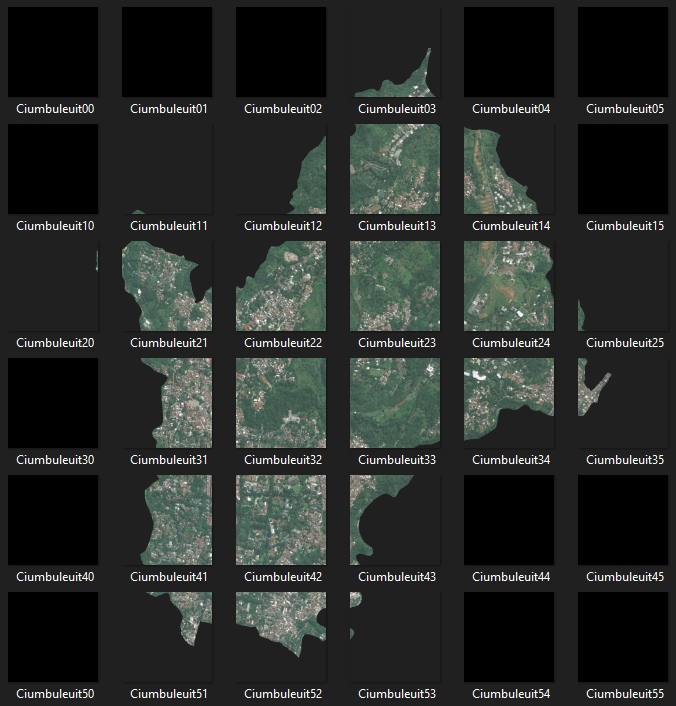
\includegraphics[width=0.5\textwidth]{Gambar/result gambar per tile.png}
	\caption{Gambar seluruh tile dari kelurahan Ciumbuleuit}
	\label{fig:pertileciumbuleuit}
\end{figure} 

\subsection{Menggabungkan Gambar}
\label{subsec:gabunggambar}
\textit{Script} yang dikembangkan dalam penelitian ini memiliki tujuan utama untuk menggabungkan sejumlah gambar per tile menjadi sebuah gambar utuh yang merepresentasikan kelurahan. Kode pemrograman dapat dilihat pada kode program \ref{code:penggabunganGambar}, menggunakan library PIL (\textit{Python Imaging Library}) dengan mengimpor kelas \textit{Image}. Terdapat beberapa variabel kunci yang ditentukan, seperti nama\_kecamatan, jumlah\_baris, dan jumlah\_kolom, yang digunakan untuk mengidentifikasi nama kelurahan serta jumlah baris dan kolom yang digunakan untuk mengatur tata letak gambar per tile.

\begin{lstlisting}[language=Python, caption=Script Penggabungan Gambar,label={code:penggabunganGambar}]
	from PIL import Image
	
	nama_kecematan = 'nama_kecamatan/kelurahan'
	jumlah_baris = 2
	jumlah_kolom = 3
	
	panjang_tile = 256
	lebar_tile = 256
	
	panjang_gambar = jumlah_kolom*panjang_tile
	lebar_gambar = jumlah_baris*lebar_tile
	
	canvas = Image.new("RGB", (panjang_gambar,lebar_gambar))
	for y in range(jumlah_baris):
	for x in range(jumlah_kolom):
	img = Image.open(nama_kecematan + str(y) + str(x) +".png")
	canvas.paste(img, (x*panjang_tile,y*lebar_tile))
	canvas.save(nama_kecematan + ".png")
	
\end{lstlisting}

Selanjutnya, variabel panjang\_tile dan lebar\_tile menentukan ukuran tile, yang dalam contoh ini adalah 256 piksel. Variabel panjang\_gambar dan lebar\_gambar dihitung berdasarkan jumlah kolom dan baris, sehingga ukuran gambar akhir dapat ditentukan. Proses pembuatan gambar  dimulai dengan inisiasi variabel canvas menggunakan fungsi \textit{Image.new }dengan mode "RGB" dan ukuran gambar sesuai dengan panjang\_gambar dan lebar\_gambar. Selanjutnya, terdapat dua \textit{loop} di mana \textit{loop} pertama digunakan untuk mengatur koordinat y, dan loop kedua untuk koordinat x. Di dalam \textit{loop-loop} tersebut, variabel img digunakan untuk membuka gambar tile yang sesuai dengan koordinatnya dengan menambahkan format file yang sesuai. Gambar yang diakses melalui variabel img kemudian disisipkan ke dalam gambar utuh \textit{canvas} menggunakan fungsi \textit{paste}. Dan terakhir, \textit{canvas.save} untuk menyimpan hasil gambar akhir dengan nama sesuai dengan 'nama\_kecamatan'. Hasil akhir gambar-gambar per tile menjadi gambar utuh yang merepresentasikan wilayah atau kecamatan yang diinginkan seperti pada gambar \ref{fig:ciumbuleuit}.

\section{Pembentukan Gambar Hasil Segmentasi}
Pada penelitian yang telah dilakukan oleh Juan Anthonius Kusjadi menghasilkan data hasil segmentasi area hijau yang telah disimpan pada sistem \textit{data lake }yang telah dibuat pada Hadoop
HDFS\cite{juan:22:pengumpulan}. Pengunduhan data gambar citra satelit hasil segmentasi area hijau kelurahan dapat dilakukan dengan kode perintah seperti pada kode \ref{code:cmdhdfssegmentasi}.

\begin{lstlisting}[language=Bash, caption= Pengembailan Data Hasil Segemntasi,label={code:cmdhdfssegmentasi}]
	hdfs dfs -get /user/if18059/geodata/result/kmeans-5/arcgis/16/Jawa_Barat/Kota_Bandung.csv .	
\end{lstlisting}

Kode Perintah \ref{code:cmdhdfssegmentasi} digunakan untuk mengunduh file CSV dari HDFS dan menyimpannya di direktori lokal tempat menjalankan perintah tersebut. Perintah \texttt{hdfs dfs -get} merupakan perintah untuk mengunduh file dari HDFS. Perintah /user/if18059/geodata/result/kmeans-5~~/arcgis/16/Jawa\_Barat/Kota\_Bandung.csv adalah jalur lengkap ke file yang ingin diunduh dari HDFS. File yang dimaksud adalah \texttt{Kota\_Bandung.csv} yang terletak di direktori /user/if18059/geodata/result/\\kmeans-5/arcgis/16/Jawa\_Barat/ di HDFS. Dan Perintah titik ("\texttt{.}") merupakan tempat menyimpan file yang diunduh ke direktori lokal.

File Kota\_Bandung.csv berisikan data hasil klasterisasi. Isi dari file Kota\_Bandung.csv memiliki 9 kolom yang dipisahkan oleh tanda titik koma (”;”). Pada kolom pertama diisi dengan nama kelurahan. Pada kolom kedua diisi dengan posisi x \textit{tile} citra satelit. Pada kolom ketiga diisi dengan posisi y \textit{tile} citra satelit. Pada kolom keempat diisi dengan nilai panjang dari \textit{tile} citra satelit pada kelurahan tersebut. Pada kolom kelima diisi dengan nilai lebar dari \textit{tile} citra satelit pada kelurahan tersebut. Pada kolom keenam diisi dengan data gambar citra satelit yang sudah disegmentasi dengan format .png berdasarkan hasil klasterisasi dan di enkripsi menggunakan Base64. Pada kolom ketujuh diisi dengan data gambar citra satelit asli dengan format .png dan di enkripsi menggunakan Base64. Pada kolom kedelapan diisi dengan nilai luas area hijau dalam km2. Terakhir pada kolom kesembilan diisi dengan nilai luas area kelurahan\cite{juan:22:pengumpulan} .

Proses pengekstrasian file Kota\_Bandung.csv berbeda dengan proses pengektrasian yang ada pada sub-bab \ref{subsec:pengkorvesianBaris} dikarenakan format file yang berbeda maka \textit{script} yang digunakan juga berbeda. Penggunaan script dapat pada file Kota\_Bandung.csv dilihat pada kode program \ref{code:ekstrakCSV}. 
\begin{lstlisting}[language=Python, caption=Script Penggabungan Gambar Hasil Klasterisasi ,label={code:ekstrakCSV}]
	import base64
	import csv
	
	def extract_image_pertile(csv_file):
		with open(csv_file, 'r') as file:
			csv_reader = csv.reader(file)
	
			for row in csv_reader:
				kelurahan = row[0]
				kordinat_x = row[1]
				kordinat_y = row[2]
				segmented_image_data = row[5]
				img_data = base64.b64decode(segmented_image_data)
				filename = f"{kelurahan}{kordinat_y}{kordinat_x}.png"
				
				with open(filename, 'wb') as img_file:
				img_file.write(img_data)
	
	
	if __name__ == "__main__":
	
	csv_file = "Kota_Bandung.csv"
	csv.field_size_limit(1000000)
	
	extract_image_pertile(csv_file)
	
	
\end{lstlisting}

\textit{Script} Python di atas dirancang untuk memproses data gambar tersegmen dalam format base64 yang terdapat dalam sebuah file Kota\_Bandung.csv. \textit{Script} ini  bertujuan untuk mengekstrak dan mendekode data gambar tersebut, kemudian menyimpannya sebagai file gambar dengan format .png. Fungsi utama yang terlibat dalam proses ini disebut \textit{extract\_image\_pertile}, yang akan menerima nama file .csv sebagai parameter. Fungsi tersebut membuka file Kota\_Bandung.csv, lalu membaca setiap baris, dan membaca nilai-nilai yang penting seperti kelurahan, koordinat x dan y, serta data gambar tersegmen yang dienkripsi dalam base64. Selanjutnya, data gambar tersebut didekode menggunakan \textit{library }base64 dan disimpan sebagai file gambar .png dengan nama sesuai dengan kelurahan yang terbentuk dari gabungan nilai-nilai kolom tertentu.

Dalam bagian utama \textit{script}, terdapat pemanggilan fungsi \textit{extract\_image\_pertile }dengan menyertakan nama file Kota\_Bandung.csv yang akan diproses. Sebagai tambahan, script ini mengatur batas ukuran untuk file .csv dengan \textit{library } csv yang telah disediakan oleh Python. Fungsi \textit{field\_size\_limit} untuk menangani batasan ukuran default yang ada. Dengan menjalankan \textit{script} ini, file gambar .png akan dihasilkan untuk setiap baris. Gambar dari setiap baris tersebut merupakan gambar pertile dari tiap kelurahan.

Setelah mendapatkan gambar per tile langkah selanjut yaitu menggabungkan gambar. Proses penggabungan gambar segmentasi area hijau sama dengan proses penggabungan gambar kelurahan sebelum segmentasi. Pada proses tersebut dapat dilihat pada sub-bab \ref{subsec:gabunggambar}.

Dalam pencarian data gambar hasil segmentasi ditemukan data berupa file Bandung.txt. Setelah melakukan pemprosesan pada data file Bandung.txt, file tersebut merupakan data file dari Kabupaten Bandung. File Bandung.txt juga memiliki beberapa kolom yang menunjukan nama kelurahan, nama kabupaten, nama provinsi, panjang tile, lebar tile, koordinat tile(x,y), data poligon, dan  \textit{tile} citra satelit yang di encode menggunakan Base64. Proses pengecekan file tersebut dilakukan dengan menggunakan \textit{script} python yang dikembangkan.

\begin{lstlisting}[language=Python, caption=Script Pengecekan File .txt,label={code:cekData}]
	#cek per satu kelurahan
	file = open("Bandung.txt","r+")
	counter = 0
	while True:
	file_line = file.readline().split(";",8)
	
	if not file.readline():
	break
	
	print(file_line[0],file_line[1],file_line[2],file_line[3],file_line[4],file_line[5],file_line[6],file_line[7])
	counter += 1

	print(counter)
	
	file.close()
\end{lstlisting}

Setelah \textit{script} \ref{code:cekData} dijalakan ternyata terdapat data yang hilang. Data yang hilang saat melakukan pengekstraksian gambar adalah beberapa \textit{tile} pada kelurahan tersebut. \textit{Tile-tile} yang hilang mengakibatkan gambar tidak dapat digabung menjadi sebuah gambar utuh dari kelurahan kabupaten. Contoh data dari Bandung.txt dapat dilihat pada gambar \ref{fig:kabupatenKopo}. Dari gambar tersebut bahwa nama kelurahan kabupaten adalah Kopo, dilanjutkan dengan nama kabupaten Bandung, provinsi Jawa Barat, lebar tile dan panjang tile. Pada kolom koordinat x dan y ada beberapa yang hilang. Data yang hilang adalah nilai x = 0, dan nilai y = 2 tidak terdapat pada kolom.
\begin{figure}[H]
	\centering
	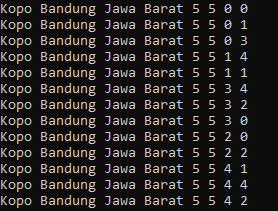
\includegraphics[width=0.5\textwidth]{Gambar/kabupatenKopo.png}
	\caption{Proses pengecekan file Bandung.txt}
	\label{fig:kabupatenKopo}
\end{figure}


\section{Pengumpulan Data Kelurahan}
\label{sec:pengambilan-data-kelurahan}
Proses pengumpulan data kelurahan yang didapatkan dari hasil penelitian yang telah dilakukan oleh Juan A. Kusjadi. Data yang ditemukan merupakan hasil perhitungan luas wilayah kelurahan dan wilayah RTH kelurahan di Kota Bandung dengan menggunakan algoritma KMeans dengan k=5 dalam pendekatan \textit{pixel based}\cite{juan:22:pengumpulan}. Hasil dari penelitian tersebut didapat dari lampiran hasil eksperimen yang berisikan nama kelurahan, luas kelurahan sesungguhnya dalam satuan km2, luas kelurahan preidiksi dalam satuan km2, luas RTH kelurahan prediksi dalam satuan km2, dan persentase RTH kelurahan.
%tambahkan foootnote tentang mysql dan xampp

Proses penginputan data dari hasil penelitian dan sumber data eksternal dilakukan secara manual dengan memasukkan data satu per satu melalui phpMyAdmin yang merupakan sebuah aplikasi berbasis web yang disediakan oleh XAMPP  untuk memudahkan dalam penyimpanan basis data MySQL. Pembuatan tabel pada MySQL dinamai dengan 'data\_wilayah'. Tabel tersebut berisikan kolom id sebagai \textit{primary key}, nama\_kelurahan, luas\_kelurahan, luas\_kelurahan\_prediksi, luas\_rth\_kelurahan dan persentase\_rth\_kelurahan. Data eksternal yang ditambahkan kedalam tabel yaitu link\_googlemaps yang berisikan tautan google maps sesuai dengan data kelurahan. 

Dengan demikian, proses pengambilan data kelurahan telah dipindahkan kedalam basis data. Data-data tersebut nantinya akan digunakan dalam pengembangan perangkat lunak.  


\section{Analisis Perangkat Lunak}
Proses analisis perangkat lunak merupakan kebutuhan yang memerlukan peranan seorang pengguna untuk menjalankan sebuah perangkat lunak yang akan dikembangkan. Sehingga segala proses sistem dijalankan oleh aktor yang terlibat. Dalam sistem ini hanya memiliki aktor sebagai \textit{user}. Seorang pemangku kepentingan atau pembuat keputusan memegang peranan sebagai \textit{user} itu sendiri. Dalam menggambarkan peranan pengguna terhadap interaksinya dengan sistem, maka dapat dilihat pada diagram \textit{use case} yang terdapat pada Gambar~\ref{fig:useCaseUser} berikut.

\begin{figure}[H]
	\centering
	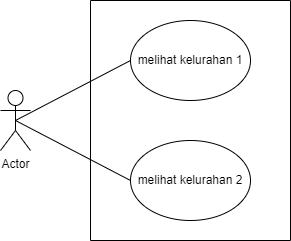
\includegraphics[scale=0.8]{Gambar/usecasediagram.png}
	\caption[Diagram \textit{Use Case} \textit{User}]{Diagram \textit{Use Case} \textit{User}}
	\label{fig:useCaseUser}
\end{figure}

Pada Gambar~\ref{fig:useCaseUser}, seorang aktor atau \textit{user} pada sistem berperan dalam memegang akses penuh ke dalam sistem. Dalam hal ini \textit{user} dapat masuk ke dalam sistem yang telah dibangun. \textit{User} dapat memilih kelurahan pertama dan kedua yang ingin dilihat. Setiap kelurahan yang dipilih \textit{user} akan menampilkan informasi luas wilayah, luas area hijau, kebutuhan area hijau, gambar citra satelit/gambar luas area hijau, dan juga dapat mengakses ke halaman \textit{Google Maps} yang merujuk ke lokasi kelurahan yang dipilih.
	
Berdasarkan diagram \textit{use case }pada Gambar \ref{fig:useCaseUser}, berikut adalah daftar skenario unutk setiap \textit{use case:}	

\begin{enumerate}
	\item Use Case: Melihat kelurahan 1 \\
	\textit{\textbf{Actor}}: Pengguna \\
	\textit{\textbf{Pre Condition: }}Pengguna telah dapat mengakses website dan berada pada halaman utama website\\
	\textit{\textbf{Post Condition:}} Pengguna melihat infromasi dari kelurahan dipilih\\
	\textit{\textbf{Steps: }}
	\begin{table}[H]
		\centering
		\resizebox{0.8\columnwidth}{!}{%
			\begin{tabular}{|l|l|}
				\hline
				\textit{\textbf{Actor Actions}}                           & \textit{\textbf{System Response}}          \\ \hline
				\multirow{2}{*}{Pengguna menekan pada dropdown kelurahan} & \multirow{2}{*}{}                          \\
				&                                            \\
				& Dropdown akan menampilakan daftar kelurahan \\
				Pengguna dapat memilih salah satu kelurahan               &                                            \\
				& Ditampilkan informasi dari kelurahan       \\ \hline
			\end{tabular}%
		}
	\end{table}
	\item Use Case: Melihat kelurahan 2 \\
	\textit{\textbf{Actor}}: Pengguna \\
	\textit{\textbf{Pre Condition: }}Pengguna telah dapat mengakses website dan berada pada halaman utama website\\
	\textit{\textbf{Post Condition:}} Pengguna melihat infromasi dari kelurahan dipilih\\
	\textit{\textbf{Steps: }}
	\begin{table}[H]
		\centering
		\resizebox{0.8\columnwidth}{!}{%
			\begin{tabular}{|l|l|}
				\hline
				\textit{\textbf{Actor Actions}}                           & \textit{\textbf{System Response}}          \\ \hline
				\multirow{2}{*}{Pengguna menekan pada dropdown kelurahan} & \multirow{2}{*}{}                          \\
				&                                            \\
				& Dropdown akan menampilakan daftar kelurahan \\
				Pengguna dapat memilih salah satu kelurahan               &                                            \\
				& Ditampilkan informasi dari kelurahan       \\ \hline
			\end{tabular}%
		}
	\end{table}
	
	\begin{comment}
	\item Use Case: Melihat luas wilayah kelurahan\\
	\textit{\textbf{Actor}}: Pengguna \\
	\textit{\textbf{Pre Condition: }}Pengguna berada pada halaman utama website dan telah memilih kelurahan yang ingin dilihat\\
	\textit{\textbf{Post Condition:}} Pengguna dapat melihat luas wilayah kelurahan yang dipilih.\\
	\textit{\textbf{Steps: }}
	\begin{table}[H]
		\centering
		\resizebox{0.8\columnwidth}{!}{%
			\begin{tabular}{|l|l|}
				\hline
				\textit{\textbf{Actor Actions}}  & \textit{\textbf{System Response}}                    \\ \hline
				Pengguna telah memilih kelurahan &                                                      \\
				& Ditampilkan informasi tentang luas wilayah kelurahan \\ \hline
			\end{tabular}%
		}
	\end{table}
	\item Use Case: Melihat luas area hijau kelurahan\\
	\textit{\textbf{Actor}}: Pengguna \\
	\textit{\textbf{Pre Condition: }}Pengguna telah dapat mengakses website dan berada pada halaman utama website\\
	\textit{\textbf{Post Condition:}} Pengguna melihat infromasi dari luas area hijau kelurahan yang dipilih\\
	\textit{\textbf{Steps: }}
	\begin{table}[H]
		\centering
		\resizebox{0.8\columnwidth}{!}{%
			\begin{tabular}{|l|l|}
				\hline
				\textit{\textbf{Actor Actions}}  & \textit{\textbf{System Response}}                    \\ \hline
				Pengguna telah memilih kelurahan &                                                      \\
				& Ditampilkan informasi tentang luas wilayah kelurahan \\ \hline
			\end{tabular}%
		}
	\end{table}
	
	
	\item Use Case: Melihat kebutuhan area hijau\\
	\textit{\textbf{Actor}}: Pengguna \\
	\textit{\textbf{Pre Condition: }}Pengguna telah dapat mengakses website dan berada pada halaman utama website\\
	\textit{\textbf{Post Condition:}} Pengguna melihat infromasi dari kebutuhan area hijau kelurahan dipilih\\
	\textit{\textbf{Steps: }}
	\begin{table}[H]
		\centering
		\resizebox{0.8\columnwidth}{!}{%
			\begin{tabular}{|l|l|}
				\hline
				\textit{\textbf{Actor Actions}}  & \textit{\textbf{System Response}}                    \\ \hline
				Pengguna telah memilih kelurahan &                                                      \\
				& Ditampilkan informasi tentang kebutuhan area hijau kelurahan \\ \hline
			\end{tabular}%
		}
	\end{table}
	
	\item Use Case: Melihat gambar citra satelit\\
	\textit{\textbf{Actor}}: Pengguna \\
	\textit{\textbf{Pre Condition: }}Pengguna telah dapat mengakses website dan berada pada halaman utama website\\
	\textit{\textbf{Post Condition:}} Pengguna melihat infromasi berupa gambar kelurahan yang dipilih\\
	\textit{\textbf{Steps: }}
	\begin{table}[H]
		\centering
		\resizebox{0.8\columnwidth}{!}{%
			\begin{tabular}{|l|l|}
				\hline
				\textit{\textbf{Actor Actions}}  & \textit{\textbf{System Response}}                    \\ \hline
				Pengguna telah memilih kelurahan &                                                      \\
				& Ditampilkan gambar citra satelit kelurahan \\ \hline
			\end{tabular}%
		}
	\end{table}
	
	\item Use Case: Mengakses ke \textit{google maps}\\
	\textit{\textbf{Actor}}: Pengguna \\
	\textit{\textbf{Pre Condition: }}Pengguna telah dapat mengakses website dan berada pada halaman utama website\\
	\textit{\textbf{Post Condition:}} Pengguna melihat infromasi berupa  \textit{link googlemaps }dari kelurahan yang dipilih\\
	\textit{\textbf{Steps: }}
	\begin{table}[H]
		\centering
		\resizebox{0.8\columnwidth}{!}{%
			\begin{tabular}{|l|l|}
				\hline
				\textit{\textbf{Actor Actions}}  & \textit{\textbf{System Response}}                    \\ \hline
				Pengguna telah memilih kelurahan &                                                      \\
				& Ditampilkan \textit{link googlemaps }kelurahan \\ \hline
			\end{tabular}%
		}
	\end{table}
	
	\item Use Case: Melihar gambar luas area hijau\\
	\textit{\textbf{Actor}}: Pengguna \\
	\textit{\textbf{Pre Condition: }}Pengguna telah dapat mengakses website dan berada pada halaman utama website\\
	\textit{\textbf{Post Condition:}} Pengguna melihat infromasi dari kelurahan dipilih\\
	\textit{\textbf{Steps: }}
	\begin{table}[H]
		\centering
		\resizebox{0.8\columnwidth}{!}{%
			\begin{tabular}{|l|l|}
				\hline
				\textit{\textbf{Actor Actions}}          & \textit{\textbf{System Response}}                  \\ \hline
				Pengguna memilih \textit{button} citra satelit    &                                                    \\
				& Ditampilkan informasi gambar dari kelurahan        \\
				Pengguna memilih \textit{button} area hijau &                                                    \\
				& Ditampilkan gambar area hijau dari kelurahan \\ \hline
			\end{tabular}%
		}
	\end{table}
	\end{comment}
\end{enumerate}
